\section{数据分析}\label{sec:dataset}

\begin{chapterquestion}
\textbf{本章研究的问题}：数据中存在哪些影响后续优化的结构性特征？
\end{chapterquestion}

\subsection{数据集来源与结构}

数据来源于 Kaggle 公开数据集
\emph{F1 Aerodynamic Stability and Porpoising (150k Samples)}。
原始约 15 万条样本经清洗后保留 104{,}999 条有效样本，
含 5 个输入特征与 1 个目标变量：输入为
$x=(\text{speed\_kmh}, \text{wing\_angle\_deg}, \text{drs\_active},
\text{downforce\_n}, \text{drag\_n})\in\mathbb{R}^5$，
目标为气动稳定性评分 $y=\text{stability\_index}\in[0,100]$。

\textbf{一个必须前置说明的事实}：该数据集并非真实 CFD 仿真，
而是由一个 XGBoost 预测引擎在 NVIDIA P100 上生成（生成器自报验证精度 99.66\%）。
这意味着数据本质是某个气动经验模型的\emph{数值近似输出}。
这一来源既解释了后文代理模型异常高的精度，
也限定了本文结论的边界——一切讨论针对"代理驱动优化"这一方法论对象，
而非真实赛车工程。

\subsection{结构特征一：严重的目标饱和（天花板效应）}

稳定性评分呈严重左偏（偏度 $-2.90$），分级分布高度不平衡：

\begin{table}[H]
\centering
\caption{稳定性分级分布}
\begin{tabular}{lrrr}
\toprule
稳定性等级 & 评分范围 & 样本数 & 占比 \\
\midrule
严重不稳定 (severe) & $[0, 30)$ & 9{,}563 & 6.38\% \\
中度不稳定 (moderate) & $[30, 60)$ & 4{,}513 & 3.01\% \\
轻度不稳定 (mild) & $[60, 95)$ & 6{,}895 & 4.60\% \\
\textbf{稳定 (stable)} & $[95, 101)$ & \textbf{129{,}028} & \textbf{86.02\%} \\
\bottomrule
\end{tabular}
\end{table}

\begin{figure}[H]
\centering
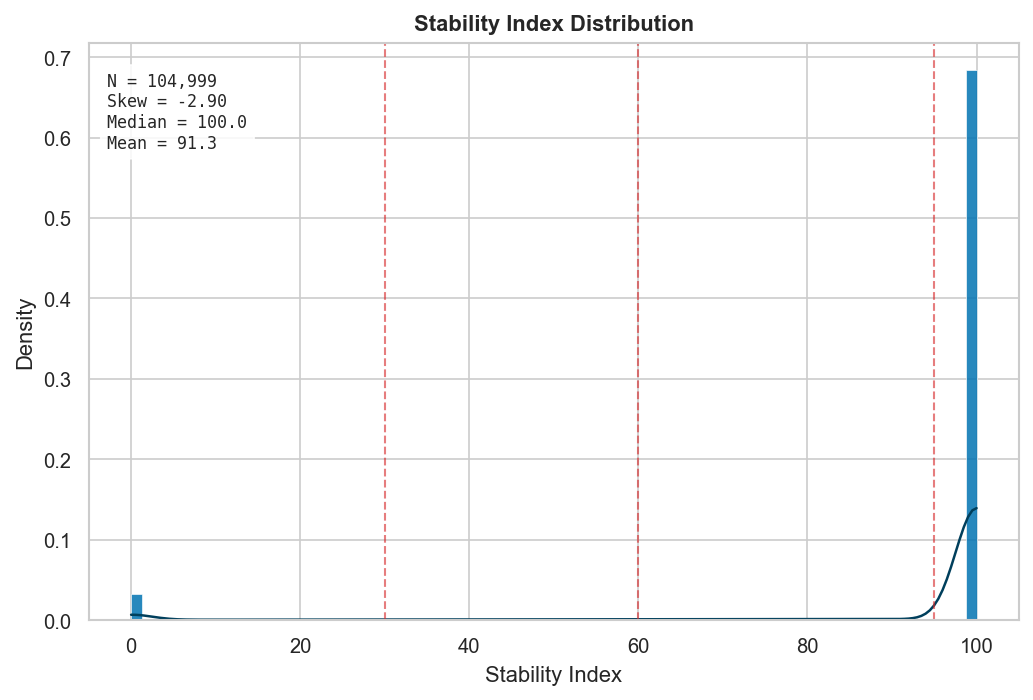
\includegraphics[width=0.78\textwidth]{figures/01_distribution.png}
\caption{各特征与稳定性评分的分布}
\label{fig:distribution}
\end{figure}

如图~\ref{fig:distribution}，绝大多数样本的稳定性集中在满分附近。
\textbf{这是第一项结构特征}：当一个目标变量的 86\% 取值趋近上界时，
任何回归代理在高稳定性区域的输出都会趋于饱和（接近一个平台），
其在该区域对输入变化的区分度将被数据本身抹平。
这一特征与第~\ref{sec:landscape}~节的景观退化分析直接相关。

针对不平衡，训练时采用类平衡加权
$w_i=N/(K\cdot n_i)$（$K=4$），
severe/moderate/mild/stable 的权重分别约为 3.92 / 8.31 / 5.44 / 0.29，
对低稳定性样本赋予更高优化优先级。

\subsection{结构特征二：强共线性与中介结构}

\begin{figure}[H]
\centering
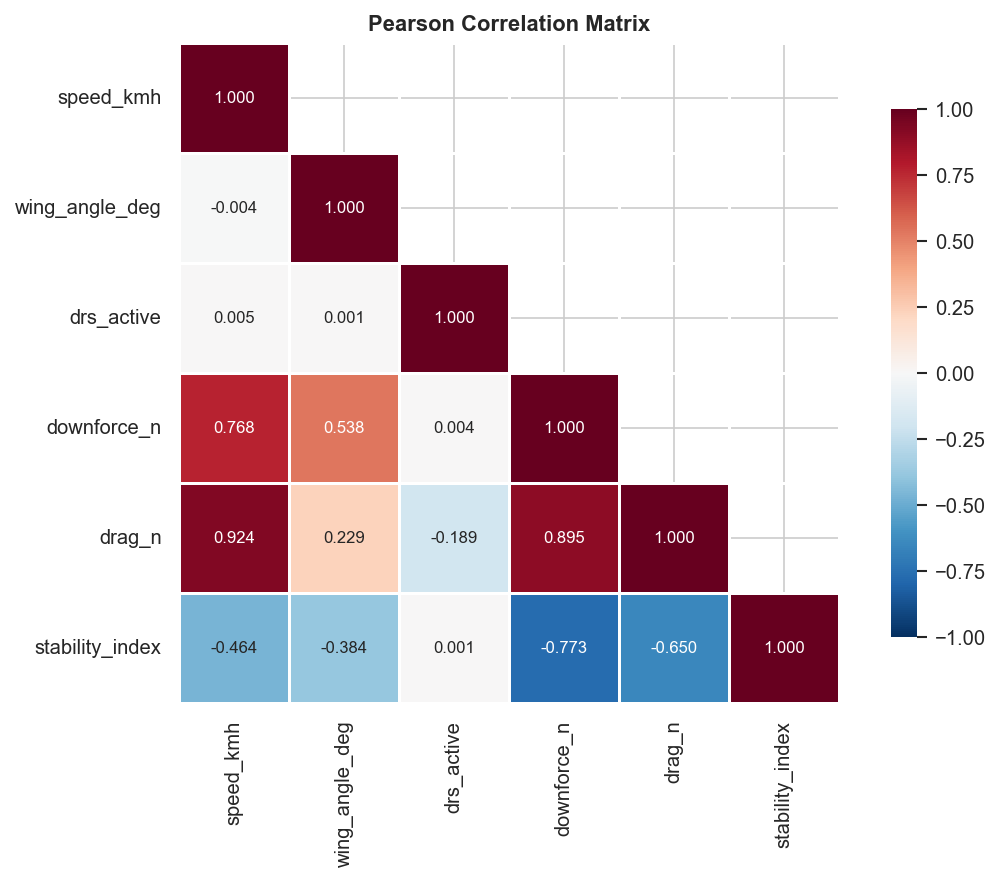
\includegraphics[width=0.72\textwidth]{figures/02_correlation.png}
\caption{特征相关系数矩阵}
\label{fig:correlation}
\end{figure}

图~\ref{fig:correlation} 揭示了第二项结构特征：
\begin{itemize}
    \item downforce\_n 与 drag\_n 之间存在\textbf{极强正相关 $r=0.895$}——
        二者几乎不可独立变化，可达解集合被结构性收窄；
    \item downforce\_n 与 stability 的相关性最强（$r=-0.773$）；
    \item wing\_angle\_deg 与 stability 的原始相关 $r=-0.384$，
        但控制 downforce 后偏相关骤降至 $0.06$——
        翼角的影响\emph{几乎完全经由下压力中介传递}；
    \item speed 与 drag（$r=0.924$）、speed 与 downforce（$r=0.768$）同样强耦合。
\end{itemize}

\textbf{两项结构特征的综合含义}：目标在高稳定区饱和（信息量低），
而特征之间高度共线（有效自由度低）。
这表明，在该数据上寻优时，最优解可能更多与\emph{数据结构}相关，
而非取决于\emph{优化能力}。下一节进入代理模型构建。

\subsection{预处理流程}

预处理包括：（1）数据清洗，剔除缺失与异常记录；
（2）特征归一化，树模型/线性模型用 StandardScaler、神经网络用 MinMaxScaler；
（3）按 $7:1.5:1.5$ 划分训练/验证/测试集（\texttt{random\_state=42}）。
